\documentclass[a4paper]{scrartcl}
\usepackage{amsmath, amsthm, amssymb}
\numberwithin{equation}{section}
\usepackage[T1]{fontenc}
\usepackage[english]{babel}
\usepackage[utf8]{inputenc}
\usepackage[parfill]{parskip}    % Activate to begin paragraphs with an empty line rather than an indent
\usepackage{graphicx}
\usepackage{caption}
\usepackage{subcaption}
\usepackage{wrapfig}
\usepackage{listings}
\usepackage{fancyhdr}
%\usepackage[]{mcode} % \lstinputlisting[firstline=300,lastline=500]{file.m}

% The report should contain:
% 1. A cover sheet with the name of the project, your names, education programs, and e-mail addresses. You must check mail to these addresses regularly.
%    Also give the date of submission and complete instructions for running your program.
% 2. An introduction (what the project is about, etc.).
% 3. Something about requirements that you fulfill or don’t fulfill.
% 4. An outline of your system (which database manager you use, which programs you have
%    written, how the programs communicate with the database, etc.).
% 5. An E/R diagram which describes the system.
% 6. Relations. Indicate primary keys, possibly secondary keys, and foreign keys. You must
%    show that the relations are normalized according to your chosen normal form (if a relation “obviously” is in BCNF you may say so,
%    provided that you  justify your statement). If a relation is in a lower normal form than BCNF, you must justify this choice.
% 7. SQL statements to create all tables, views, stored procedures, and other database elements.
%    (Don’t include statements to create the initial contents of the database.)
% 8. A user’s manual (not necessary if everything in the program is self-explanatory).


\pagestyle{fancy}
\thispagestyle{empty}
\rhead{Johannes Jansson and Victor Miller}
\lhead{}

\begin{document}

\title{Programming Project: Krusty Cookies}
\author{Johannes Jansson, F11\\tfy11jja@student.lu.se\\\\Victor Miller, F11\\tfy11vmi@student.lu.se}

\date{}
\maketitle
\newpage

\section*{Introduction}
\section*{Requirements}
Even though the requirements were a bit diffuse (as intended) we are fairly confident that we have met all of them. 
\section*{Outline of the System}
\section*{E/R Diagram}

\begin{figure}[h!]
  \begin{centering}
    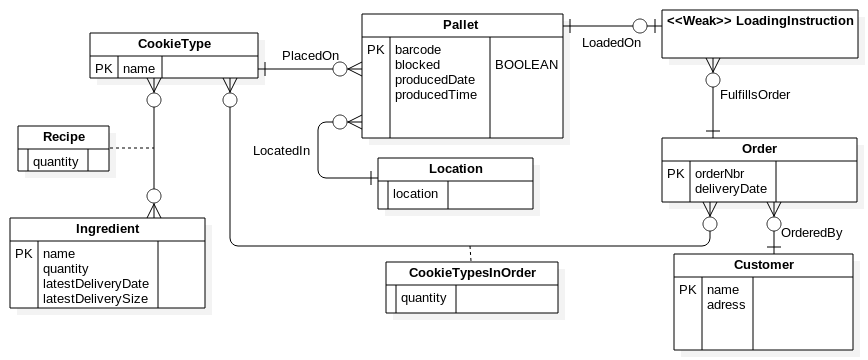
\includegraphics[width=\textwidth]{../ER.png}
    \label{er-diagram}
    \caption{E/R--diagram for the system}
  \end{centering}
\end{figure}

\section*{Relations}
The following relations were the basis for creating the database:

\lstinputlisting[firstline=21]{../Relations.txt}
\section*{SQL Statements}
The following SQL statements were used to create the database:

\lstinputlisting[lastline=83]{../tables.sql}
\section*{User's manual}
We consider the system self--explanatory enough not to require an user manual. 
The system has, in fact, been tested on a med--student with great success.
The only things worth pointing out are that:

\begin{enumerate}
  \item This thing
  \item This thing
  \item And this thing
\end{enumerate}

% % Task 1
% \setcounter{section}{1}
% \section*{Task 1}
% \input{../task1/task1.tex}






% \begin{thebibliography}{9}
    
%   \bibitem{cb}
%     B. Kolman, R. E. Beck, \emph{Elementary Linear Programming with Applications}.
%     2nd edition. Academic Press, San Diego, 1995,

% \end{thebibliography}

\end{document}
